\documentclass[12pt]{report}
\usepackage[top=1in, bottom=1in, left=0.5in, right=0.5in]{geometry}
\usepackage{amsmath, amsfonts, amssymb, ebgaramond-maths, enumerate, fancyhdr, xcolor, lipsum, titling, minted, algorithm, algpseudocode, algorithmicx, float, hyperref, booktabs, graphicx}
\usepackage[utf8]{inputenc}

\usepackage[Glenn]{fncychap}
\usepackage[skip=20pt, indent=30pt]{parskip}
\usepackage{setspace}
\onehalfspacing

\usepackage[some]{background}

\definecolor{titlepagecolor}{cmyk}{.02,.04,0,.90}

\DeclareFixedFont{\bigsf}{T1}{phv}{b}{n}{1.5cm}
% Default fixed font does not support bold face
\DeclareFixedFont{\ttb}{T1}{txtt}{bx}{n}{12} % for bold
\DeclareFixedFont{\ttm}{T1}{txtt}{m}{n}{12}  % for normal

% Custom colors
\usepackage{color}
\definecolor{deepblue}{rgb}{0,0,0.5}
\definecolor{deepred}{rgb}{0.6,0,0}
\definecolor{deepgreen}{rgb}{0,0.5,0}

\usepackage{listings}

% Python style for highlighting
\newcommand\pythonstyle{\lstset{
language=Python,
basicstyle=\ttm,
morekeywords={self},              % Add keywords here
keywordstyle=\ttb\color{deepblue},
emph={MyClass,__init__},          % Custom highlighting
emphstyle=\ttb\color{deepred},    % Custom highlighting style
stringstyle=\color{deepgreen},
frame=tb,                         % Any extra options here
showstringspaces=false,
tabsize=2,
}}


% Python environment
\lstnewenvironment{python}[1][]
{
\pythonstyle
\lstset{#1}
}
{}

% Python for external files
\newcommand\pythonexternal[2][]{{
\pythonstyle
\lstinputlisting[#1]{#2}}}

% Python for inline
\newcommand\pythoninline[1]{{\pythonstyle\lstinline!#1!}}


\makeatletter
\renewcommand{\@chapapp}{Section}
\makeatother
\renewcommand{\thechapter}{\Roman{chapter}}

\pagestyle{fancy}
\fancyhead[l]{Final Project Report \\}
\fancyhead[c]{Section \thechapter \\}
\fancyhead[r]{Sayan Das: \texttt{B2430035} \\ Raihan Uddin: \texttt{B2430070}}
\fancyfoot[c]{\thepage}
\renewcommand{\headrulewidth}{0.2pt}
\setlength{\headheight}{28pt}

\title{Final Project Report}
\author{
  Sayan Das
  \and
  Raihan Uddin
}

\begin{document}

\begin{titlepage}
	\newcommand{\HRule}{\rule{\linewidth}{0.5mm}}
	\center


	\textsc{\LARGE \textbf{Ramakrishna Mission Vivekananda Educational and Research Institute}}\\[1.5cm]

	\textsc{\LARGE Machine Learning}\\[0.5cm]

	\textsc{\large Final Project Report}\\[0.5cm]

	\HRule\\[0.4cm]

	{\huge\bfseries A Classification Based approach for predicting Smartphone Price Categories}\\[0.4cm]

	\HRule\\[1.5cm]



	\begin{minipage}{0.4\textwidth}
		\begin{flushleft}
			\large
			\textit{Submitted By}\\
			\textsc{\textbf{Sayan Das }}\\
			\vspace{-0.5em}
			\textsc{\texttt{B2430035 }}\\
			\textsc{\textbf{Raihan Uddin }}\\
			\vspace{-0.5em}
			\textsc{\texttt{B2430070} }\\
		\end{flushleft}
	\end{minipage}
	~
	\begin{minipage}{0.4\textwidth}
		\begin{flushright}
			\large
			\textit{Submitted To}\\
			\textbf{\textsc{Br. Bhaswarachaitanya (Tamal Maharaj)}}
		\end{flushright}
	\end{minipage}


	\vfill\vfill\vfill

	{\large November 25, 2024}

	\vfill

\end{titlepage}
\restoregeometry

\tableofcontents

\chapter{Introduction}
\section{Background}
Now a days, smartphones are more than just a means of communication. The global smartphone market is characterized by rapid technological innovation, intense competition, and increasingly sophisticated consumer expectations. With the proliferation of smartphones, the market dynamics have become increasingly complex, driven by continuous technological advancements, changing consumer preferences, and competitive pricing strategies.

The smartphone industry represents a highly dynamic technological ecosystem where manufacturers constantly strive to differentiate their products through innovative features, design, and pricing. Each season, hundreds of new smartphones are launched, each targeting different market segments and consumer needs. This rapid evolution creates significant challenges for both manufacturers and consumers in understanding and predicting smartphone pricing.

From a manufacturer's perspective, optimal pricing is crucial for maintaining market competitiveness and profitability. Pricing strategies must balance multiple factors including technological features, production costs, market positioning, and consumer purchasing power. Inaccurate pricing can lead to significant market share losses or reduced profit margins.

For consumers, purchasing a smartphone requires understanding of the complex landscape of technical specifications, brand reputation, and market trends. The ability to predict or understand the factors influencing smartphone prices can help consumers make more informed purchasing decisions and assess the value proposition of different devices.

The emergence of machine learning techniques offers promising approaches to address these pricing challenges. By leveraging historical data and advanced predictive modeling, it becomes possible to develop more sophisticated and accurate methods of smartphone price categorization and prediction.
\section{Motivation}
The motivation for this research stems from the increasingly complex and dynamic nature of the smartphone market. Several critical challenges drive the need for an advanced smartphone price categorization approach:
\vspace{-1.25em}
\begin{enumerate}
	\setlength\itemsep{-1.05em}
	\item{\textbf{Economic Significance for Manufacturers :}} Inaccurate pricing can result in significant financial losses or missed market opportunities.
	\item{\textbf{Tranceparent Pricing for Consumers :}} Many consumers face challenges in understanding the intrinsic value of smartphones. A data-driven approach to price categorization can provide transparent insights into the factors that genuinely influence smartphone pricing.
\end{enumerate}
\section{Objectives}
The primary objectives of this project are:
\vspace{-1.25em}
\begin{enumerate}
	\setlength\itemsep{-1.05em}
	\item{\textbf{Develop a Robust Classification Model :}}
		\vspace{-1.65em}
		\begin{itemize}
			\setlength\itemsep{-1.5em}
			\item Create a machine learning model capable of accurately categorizing smartphones into distinct price segments
			\item Achieve high predictive accuracy using multiple classification algorithms
			\item Identify and leverage the most significant features influencing smartphone pricing
		\end{itemize}
	\item{\textbf{Feature Analysis and Selection :}}
		\vspace{-1.65em}
		\begin{itemize}
			\setlength\itemsep{-1.5em}
			\item Conduct comprehensive analysis of smartphone features
			\item Determine the most influential factors in price categorization
			\item Develop a systematic approach to feature selection and importance ranking
		\end{itemize}
	\item{\textbf{Comparative Algorithm Performance :}}
		\vspace{-1.65em}
		\begin{itemize}
			\setlength\itemsep{-1.5em}
			\item Implement and evaluate multiple machine learning algorithms
			\item Compare the performance of different classification techniques
			\item Identify the most effective algorithm for smartphone price category prediction
		\end{itemize}
	\item{\textbf{Practical Applicability :}}
		\vspace{-1.65em}
		\begin{itemize}
			\setlength\itemsep{-1.5em}
			\item Demonstrate the practical utility of the developed model for both manufacturers and consumers
		\end{itemize}
	\item{\textbf{Methodological Contribution :}}
		\vspace{-1.65em}
		\begin{itemize}
			\setlength\itemsep{-1.5em}
			\item Develop a systematic approach to smartphone price categorization
			\item Contribute to the existing body of knowledge in machine learning applications in market analysis
			\item Establish a replicable methodology for similar predictive modeling challenges
		\end{itemize}
\end{enumerate}

\chapter{Literature Review}
\begin{quotation}
  In this paper \cite{asim2018} the authors investigate price class prediction for smartphones using machine learning, focusing on determining whether a smartphone is economical or expensive. Data was collected from GSMArena, including features like display size, weight, RAM, and battery capacity. The dataset was preprocessed and categorized into four price classes: very economical, economical, expensive, and very expensive. Feature selection methods like InfoGain and WrapperAttributeEval were employed to reduce dataset dimensionality, optimizing computational efficiency. The study tested classifiers such as Decision Tree (J48) and Naïve Bayes, achieving a maximum accuracy of 78\% with Decision Tree when combined with WrapperAttributeEval. Challenges included converting a regression problem into classification, which introduced errors, and the limited dataset size impacting accuracy. The paper concludes with recommendations for improved feature selection techniques, larger datasets, and extending the model for other product categories.
\end{quotation}

\begin{quotation}
  Chandrashekhara et al. \cite{chandrashekhara2019} 2019, focuses on predicting smartphone prices using machine learning techniques like Support Vector Regression (SVR), Backpropagation Neural Network (BNN), and Multiple Linear Regression (MLR). The dataset included features such as brand, RAM, memory, battery power, and display size, with 262 records spanning 2010–2018, sourced from e-commerce platforms. Data preprocessing steps included handling missing values, standardizing formats, and splitting the data into training (80\%) and testing (20\%) sets. Performance metrics such as R-squared and correlation values were used to evaluate models. SVR performed the best with an R-squared of 0.86 and correlation of 0.93. Graphical analyses demonstrated that SVR had the most accurate predictions, followed by BNN and MLR. The authors highlight the potential of SVR for broader applications in price prediction across retail industries, suggesting scalability through distributed systems like Hadoop.
\end{quotation}

\begin{quotation}
  Ercan \& Şimşek \cite{ercan2023} examines the classification of smartphone prices into low, medium, high, and very high categories using a Kaggle dataset with 2000 entries and 20 features. Features included physical attributes (weight, dimensions), performance metrics (RAM, processor cores), and functionalities (3G, Wi-Fi). Four machine learning algorithms—Logistic Regression, Support Vector Machine (SVM), Decision Tree, and K-Nearest Neighbors (KNN)—were applied and evaluated. SVM achieved the highest accuracy (96.16\%), outperforming Logistic Regression (91\%), Decision Tree (82\%), and KNN (41\%). Confusion matrices and performance metrics (accuracy, precision, recall, and F1-score) were used to validate results. The study emphasizes the superiority of SVM for this classification problem and suggests exploring additional algorithms and datasets for improved accuracy in future work.
\end{quotation}

\begin{quotation}
  In another study \cite{abbasi2024} the author focuses on predicting the price of second-hand electronic devices, particularly smartphones, using machine learning (ML) techniques. It addresses the growing trend of buying used electronics, driven by economic factors and technological advancements. The authors utilized web scraping to gather a dataset covering the last five years, containing various features influencing smartphone prices. They experimented with three ML algorithms—Random Forest, Linear Regression, and Multi-Layer Perceptron—to develop a predictive model. Performance evaluation was based on metrics like Absolute Percentage Difference (APD) and Root Mean Square Error (RMSE). Random Forest emerged as the best-performing model, demonstrating the lowest prediction error and superior generalization. The study highlights how accurate price prediction can aid both buyers and sellers, making the market more efficient. Data preprocessing and feature selection were critical steps, leading to a dataset with 24 variables. Techniques like 10-fold cross-validation were used to ensure robustness. The findings suggest that incorporating modern ML methods can significantly enhance price prediction accuracy compared to traditional approaches.
\end{quotation}

\begin{quotation}
  In this paper  Akash Gupta, and Suhasini Kottur \cite{gupta2020} explore smartphone price prediction using machine learning, aiming to categorize smartphones as economical or expensive based on their features. The study emphasizes the relevance of predictive modeling in aiding marketing and consumer decision-making. Key features considered include processor type, battery capacity, memory, and screen size. The authors employed algorithms like Linear Regression and K-Nearest Neighbors (KNN) to build predictive models. The seven-step machine learning process involved data gathering, preparation, model selection, training, evaluation, hyperparameter tuning, and prediction. The KNN model showed higher accuracy compared to Linear Regression, particularly in scenarios involving complex, non-linear relationships. The research demonstrated the importance of feature selection to reduce computational complexity and enhance prediction precision. The conclusion underscores the impact of ML-driven price prediction in optimizing marketing strategies and enhancing business decisions.
\end{quotation}

\begin{quotation}
  Finally, this paper \cite{kumuda2021} investigates the prediction of smartphone prices using machine learning, with a focus on market analysis and consumer behavior. The study outlines the challenges of determining accurate smartphone prices due to diverse features and competitive market dynamics. A dataset containing information on screen size, memory, camera quality, and battery was used to train predictive models. Key algorithms employed included KNN, Forward Selection, and Backward Selection to manage data complexity and optimize feature selection. The data collection phase involved gathering specifications from various smartphones to construct a comprehensive dataset. The authors emphasized the role of data visualization techniques, like the Elbow Method, to identify the optimal number of features. The study presented a detailed analysis of feature importance, highlighting key parameters influencing price prediction. Classification and testing phases assessed the model's accuracy, using preprocessed datasets for training and evaluation. Results were visualized using graphs that compared predicted prices against specifications like RAM and memory. The conclusion suggests that precise feature selection can improve predictive accuracy and aid in product launch decisions.
\end{quotation}


\chapter{Dataset Description}
\section{Source}
The dataset for this smartphone price classification project was obtained from Kaggle, a prominent platform for data science and machine learning datasets.\\ \\
Link - \href{https://www.kaggle.com/datasets/iabhishekofficial/mobile-price-classification?select=train.csv}{https://www.kaggle.com/datasets/iabhishekofficial/smartphone-price-classification}\\ \\
The dataset is publicly available and contains 2000 smartphone entries with 20 feature variables and a target variable representing price range.
\section{Features}
The dataset comprises 20 features that describe various characteristics of smartphones. Following table provides a detailed breakdown of these features:
\begin{table}[H]
	\begin{tabular}{lll}
		\toprule
		\textbf{Feature Name}   & \textbf{Description}  & \textbf{Type}  \\
		\toprule
		\textbf{battery\_power} & battery capacity in mAh   & Numerical  \\
		\midrule
		\textbf{blue}           & has bluetooth or not  & Binary   \\
		\midrule
		\textbf{clock\_speed}   & speed at which processor executes instructions & Numerical \\
		\midrule
		\textbf{dual\_sim}      & has dual sim support or not & Binary \\
		\midrule
		\textbf{fc}             & front Camera Megapixels & Numerical \\
		\midrule
		\textbf{pc}             & primary Camera Megapixels & Numerical \\
		\midrule
		\textbf{four\_g}        & has 4G or not & Binary \\
		\midrule
		\textbf{three\_g}       & has 3G or not & Binary \\
		\midrule
		\textbf{wifi}           & has wifi or not & Binary \\
		\midrule
		\textbf{int\_memory}    & internal Memory capacity & Numerical \\
		\midrule
		\textbf{m\_dep}         & smartphone Depth in cm & Numerical \\
		\midrule
		\textbf{mobile\_wt}     & weight of the smartphone & Numerical \\
		\midrule
		\textbf{n\_cores}       & number of cores in processor & Numerical \\
		\midrule
		\textbf{px\_height}     & pixel Resolution Height & Numerical \\
		\midrule
		\textbf{px\_width}      & pixel Resolution Width & Numerical \\
		\midrule
		\textbf{ram}            & RAM in MB & Numerical \\
		\midrule
		\textbf{touch\_screen}  & has touch screen or not & Binary \\
		\midrule
		\textbf{sc\_h}          & screen Height in cm & Numerical \\
		\midrule
		\textbf{sc\_w}          & screen Width in cm & Numerical \\
		\midrule
		\textbf{talk\_time}     & longest time that a single battery charge will last over a call & Numerical \\
		\bottomrule
	\end{tabular}
\end{table}
Among these features, some are binary variables (e.g., blue, dual\_sim, four\_g, three\_g touch\_screen, wifi), while others are continuous variables (e.g., battery\_power, clock\_speed, int\_memory, ram, talk\_time). These features collectively provide a comprehensive overview of the smartphone's technical specifications and capabilities.
\section{Target Variable}
The target variable, price\_range, represents the categorization of smartphones into different price segments. It is a categorical variable with four distinct classes:
\vspace{-1.25em}
\begin{itemize}
	\setlength\itemsep{-1.05em}
	\item{\texttt{0 :}} Low-cost smartphones
	\item{\texttt{1 :}} Medium-low cost smartphones
	\item{\texttt{2 :}} Medium-high cost smartphones
	\item{\texttt{3 :}} High-end, premium smartphones
\end{itemize}

\chapter{Data Preprocessing}
\section{Data Cleaning}
\subsection{Handling Missing Values}
A check for missing values - \pythoninline{df.isnull().sum()} revealed no missing values in the dataset.
\begin{python}
battery_power    0
blue             0
clock_speed      0
dual_sim         0
fc               0
four_g           0
int_memory       0
m_dep            0
mobile_wt        0
n_cores          0
pc               0
px_height        0
px_width         0
ram              0
sc_h             0
sc_w             0
talk_time        0
three_g          0
touch_screen     0
wifi             0
price_range      0
dtype: int64
\end{python}
\subsection{Handling Duplicate Values}
Also, the dataset was checked for duplicate entries - \pythoninline{df.duplicated().sum()}. No duplicate entries were found.
\begin{python}
np.int64(0)
\end{python}
\subsection{Handling Invalid Values}
The dataset was checked for negative entries with
\begin{python}
negative_counts = df.apply(lambda x: (x < 0).sum())
print(negative_counts)
\end{python}
\begin{python}
battery_power    0
blue             0
clock_speed      0
dual_sim         0
fc               0
four_g           0
int_memory       0
m_dep            0
mobile_wt        0
n_cores          0
pc               0
px_height        0
px_width         0
ram              0
sc_h             0
sc_w             0
talk_time        0
three_g          0
touch_screen     0
wifi             0
price_range      0
dtype: int64
\end{python}
No negative values were found in the dataset.

\noindent There are some features which can not be zero, like battery\_power, ram, etc. So, we checked for zero values in these features.
\begin{python}
zero_counts = df.apply(lambda x: (x == 0).sum())
print(zero_counts)
\end{python}
\begin{python}
battery_power       0
blue             1010
clock_speed         0
dual_sim          981
fc                474
four_g            957
int_memory          0
m_dep               0
mobile_wt           0
n_cores             0
pc                101
px_height           2
px_width            0
ram                 0
sc_h                0
sc_w              180
talk_time           0
three_g           477
touch_screen      994
wifi              986
price_range       500
dtype: int64
\end{python}
We can see px\_height and sc\_w are have 2 and 180 zero values respectively. We will replace these zero values with the mean of the respective features.
\begin{python}
to_replace_with_mean = ['sc_w', 'px_height']

for feature in to_replace_with_mean:
	df[feature] = df[feature].replace(0, df[feature].mean())
\end{python}
Note that fc and pc are numerical yet zero values are not invalid. They can be zero if the phone does not have a front or primary camera.

\section{Outlier Handling}
Outliers can significantly impact the performance of machine learning models. To identify and handle outliers, box plots were generated for each feature to visualize the distribution of data points. \\
\begin{figure}[H]
	\centering
	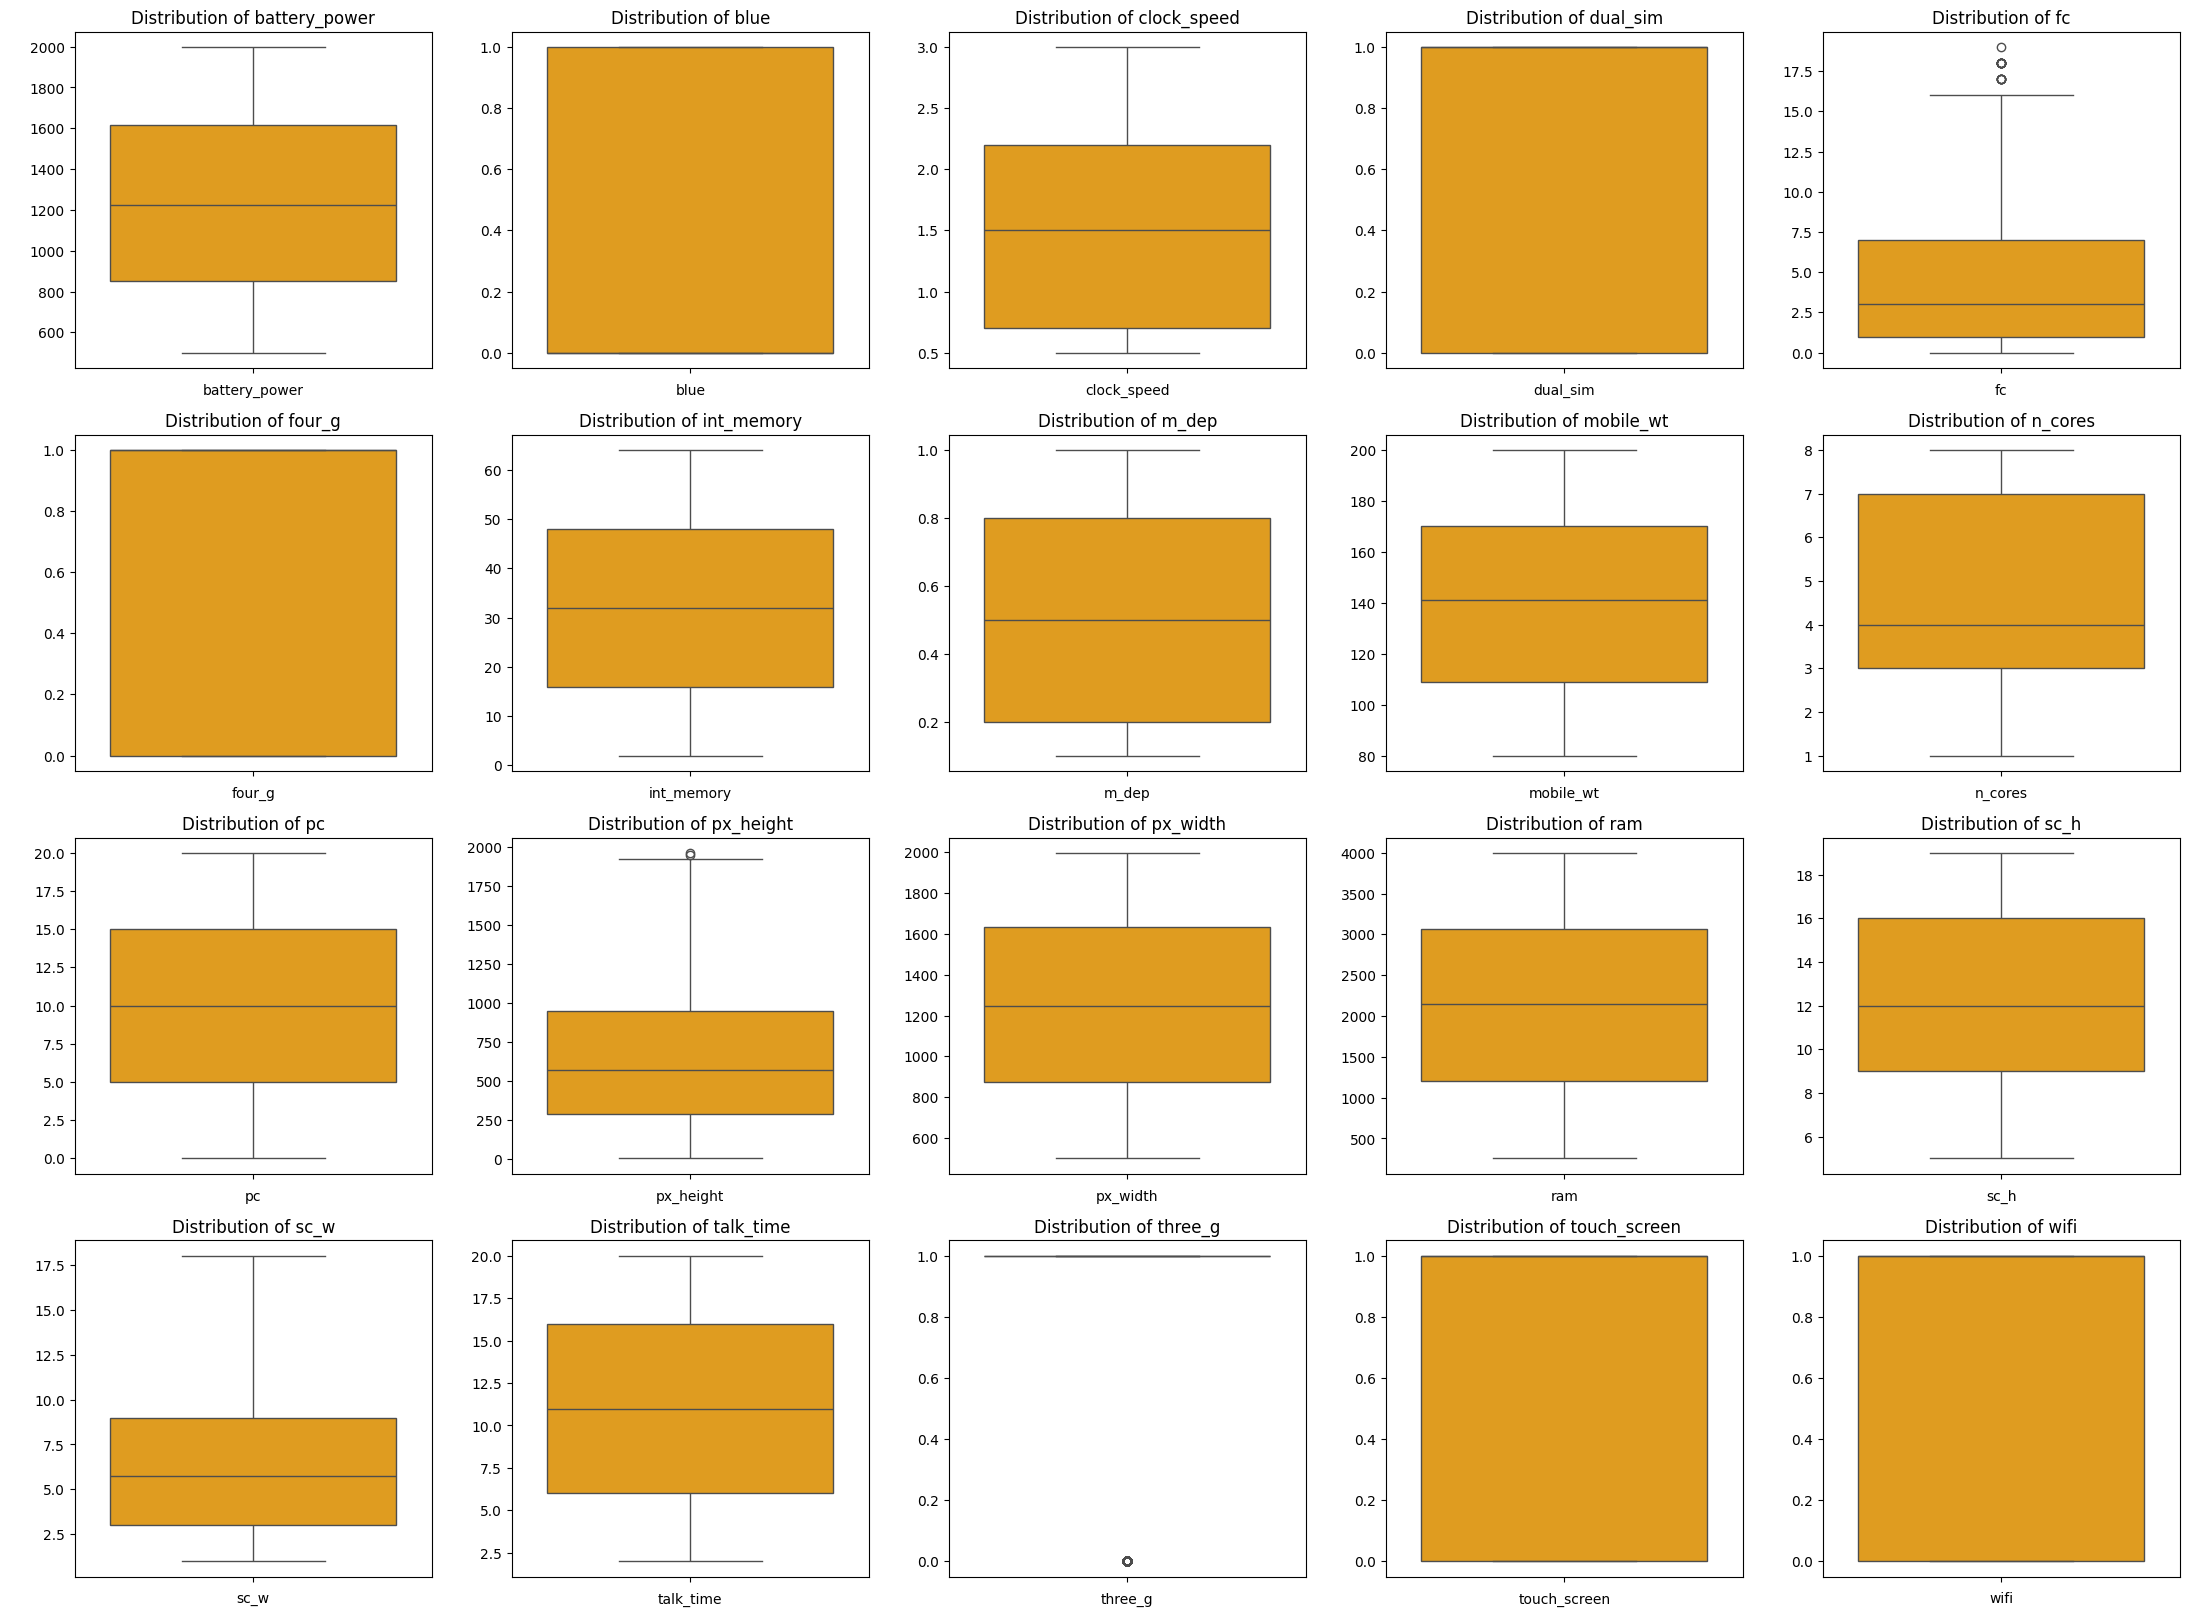
\includegraphics[height=25em]{box_plots_before.png}
	\caption{Box plots of features before outlier handling.}
	\label{box_plots_before}
\end{figure}
The box plots revealed outliers in two features, fc and px\_height. To address these outliers, the IQR (Interquartile Range) method was used to detect and remove extreme values.
\begin{figure}[H]
	\centering
	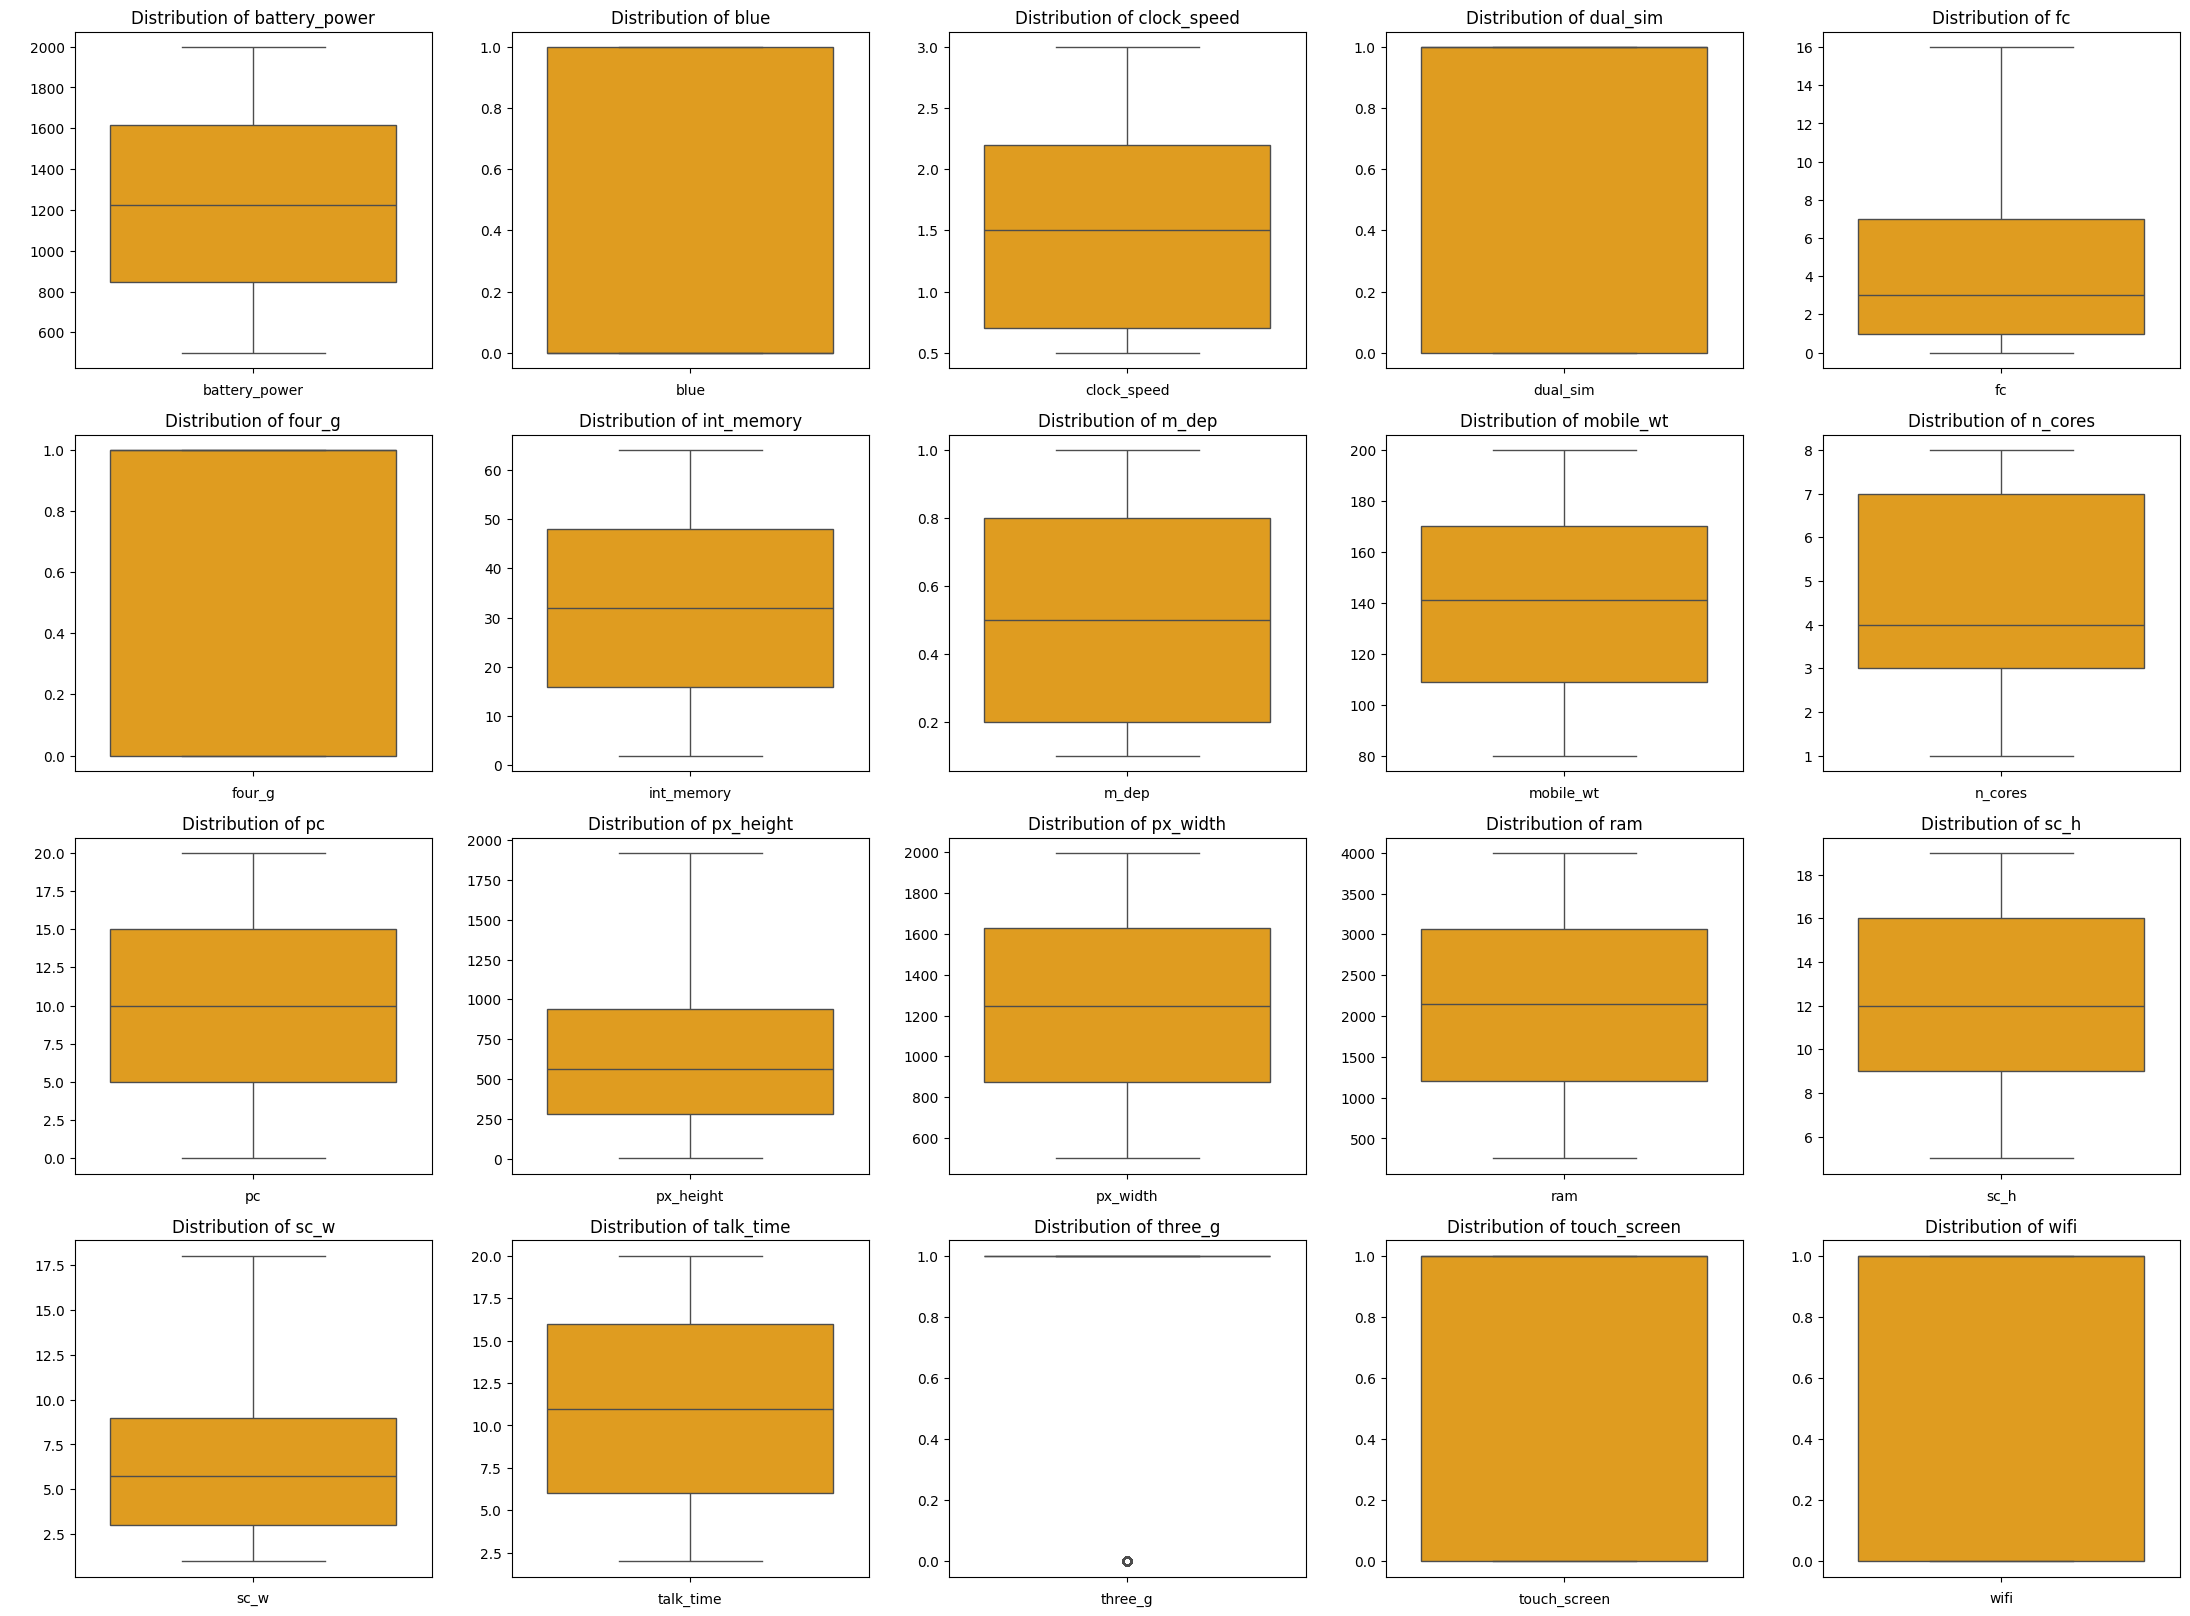
\includegraphics[height=25em]{box_plots_after.png}
	\caption{Box plots of features after outlier handling.}
	\label{box_plots_after}
\end{figure}
\section{Class Imbalance Check}
Class imbalance can affect the performance of classification models. To check for class imbalance, the distribution of the target variable was visualized using a count plot.
\begin{figure}[H]
	\centering
	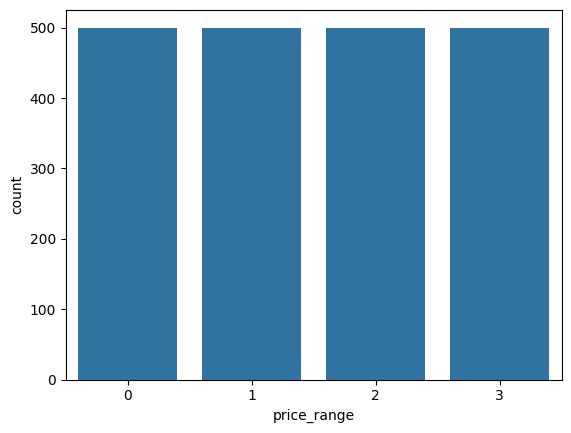
\includegraphics[height=10em]{imbalance_check.png}
	\caption{Class imbalance check for target variable.}
	\label{imbalance_check}
\end{figure}
The count plot revealed that the dataset was balanced across all four price range categories, with an equal distribution of samples in each class.
\section{Correlation Analysis}
A correlation matrix was generated to identify the relationships between different features and the target variable. This analysis helped identify the most influential features in predicting smartphone prices. The correlation matrix was visualized using a heatmap to provide a clear overview of feature relationships.
\begin{figure}[H]
	\centering
	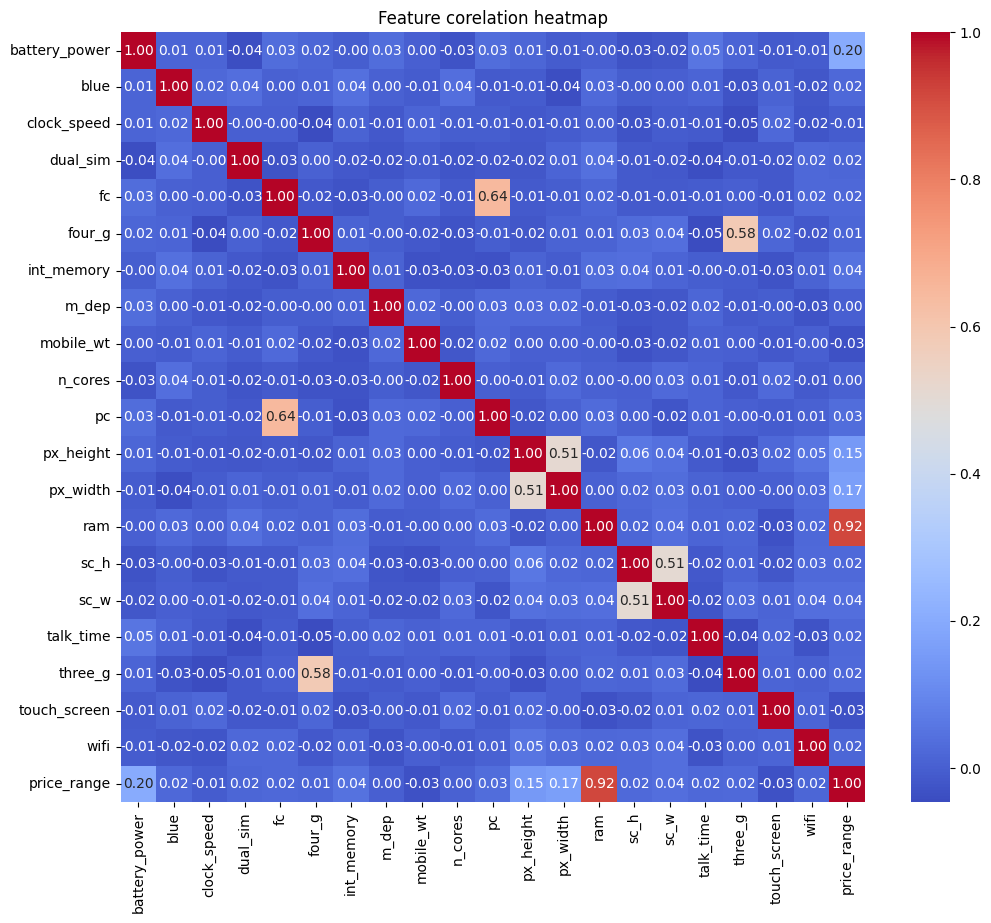
\includegraphics[height=35em]{corr_viz.png}
	\caption{Correlation heatmap of features.}
	\label{corr_viz}
\end{figure}
Here we can see that ram is highly correlated with price range. There are some features which are correlated with each other like:
\vspace{-1.25em}
\begin{enumerate}
	\setlength\itemsep{-1.05em}
	\item{\textbf{3G and 4G :}} A high correlation here suggests that devices with 4G almost always support 3G, making one of these features redundant.
	\item{\textbf{fc and pc :}} These features are correlated, as better primary cameras often accompany better front cameras.
	\item{\textbf{px\_height and px\_width :}} These are components of screen resolution and are naturally correlated.
	\item{\textbf{sc\_h and sc\_w :}} These are also naturally correlated.
\end{enumerate}
These correlations will be taken into note during next steps to reduce feature redundancy and improve model performance.
\section{Feature Engineering}
Feature engineering involved creating new features from existing ones to enhance the dataset's predictive power. The goal was to derive meaningful attributes that capture relationships between variables and optimize the dataset for machine learning model training. Two new features were introduced based on the existing data:
\vspace{-1.25em}
\begin{enumerate}
	\setlength\itemsep{-1.05em}
	\item{\textbf{px\_area :}} The total pixel area of the smartphone screen, calculated as the product of pixel resolution height (px\_height) and pixel resolution width (px\_width).
	\begin{python}
	df['px_area'] = df['px_height'] * df['px_width']
	\end{python}
	\item{\textbf{screen\_area :}} The physical screen area of the smartphone, calculated as the product of screen height (sc\_h) and screen width (sc\_w).
	\begin{python}
	df['screen_area'] = df['sc_h'] * df['sc_w']
	\end{python}
\end{enumerate}
After deriving the new features, the original components (px\_height, px\_width, sc\_h, sc\_w) were removed from the dataset:
\begin{python}
df.drop(['px_height', 'px_width', 'sc_h', 'sc_w'], axis=1, inplace=True)
\end{python}
Next, based on correlation analysis, the following redundant features were removed:
\vspace{-1.25em}
\begin{itemize}
	\setlength\itemsep{-1.05em}
	\item A high correlation exists between 3G and 4G, as devices with 4G generally support 3G. The 4G feature was retained, and 3G was removed.
	\begin{python}
	df = df.drop(['three_g'], axis=1)
	\end{python}
	\item Front and primary cameras are correlated, as primary cameras often accompany front cameras. The pc feature was retained, and fc was removed.	
	\begin{python}
	df = df.drop(['fc'], axis=1)
	\end{python}
\end{itemize}

\section{Feature Selection}
We preformed feature selection to identify the most relevant features for predicting smartphone prices. This step involved analyzing feature importance scores from machine learning models, conducting correlation analysis, and using domain knowledge to select the most influential features. Feature selection is aimed to reduce model complexity and improve prediction accuracy.

\noindent In our project, we used the ANOVA F-test (Analysis of Variance) method to evaluate each feature's relationship with the target variable, price\_range, and select features that are statistically significant. The threshold for selection is a p-value of less than $0.05$, indicating $95\%$ confidence. \\
The \pythoninline{SelectKBest} method from \pythoninline{sklearn.feature_selection} is used with the scoring function \pythoninline{f_classif}, which applies the ANOVA F-test. \\
Initially, \pythoninline{k='all'} is set to retain all features for evaluation, allowing for the computation of statistical metrics across all features. \\
After fitting the model, the p-values and F-scores for each feature are extracted. These metrics help assess the significance and contribution of each feature to the target variable. \\
Features with a p-value less than $0.05$ are considered statistically significant and are selected for further analysis. \\
The selected features are \pythoninline{['battery_power', 'int_memory', 'mobile_wt', 'n_cores', 'ram', 'px_area']} \\
These are then used for model training and evaluation to determine their impact on prediction accuracy and model performance.


\section{Train-Test Split}
\label{sec:train_test_split}
The dataset was split into training and testing sets to evaluate model performance. The training set was used to train the machine learning models, while the testing set was used to assess model accuracy and generalization. The split ratio was 80\% training and 20\% testing to ensure an adequate balance between model training and evaluation. We used sklearn's \pythoninline{train_test_split} function to perform the split.
\section{Data Transformation}
Data transformation involved feature scaling to normalize the data and improve model performance. This step ensured that all features were in a suitable format for machine learning model training. We used a pipeline to apply transformations consistently across training and test sets:
\begin{python}
from sklearn.pipeline import Pipeline
from sklearn.preprocessing import StandardScaler, PowerTransformer

pipeline = Pipeline([
    ('normalizer', PowerTransformer()),
    ('scaler', StandardScaler())
])

pipeline.fit(X_train)

X_train_scaled = pipeline.transform(X_train)
X_test_scaled = pipeline.transform(X_test)
\end{python}

\chapter{Methodology}
\section{Algorithms Used}
For this project, we experimented with several machine learning algorithms to predict smartphone price categories. The following algorithms were implemented and evaluated:
\vspace{-1.25em}
\begin{enumerate}
	\setlength\itemsep{-1.05em}

\item{\textbf{Logistic Regression: }}Logistic Regression allows us to predict the probability of the dependent variable from a given set of independent variables. The probability values are between 0 and 1. \cite{hadsonml}
\item{\textbf{Support Vector Machine: }}In Support Vector Machine, the data is separated into two classes and placed on a plane known as the marginal plane. Points from two classes that are adjacent to the line are called support vectors. The goal of Support Vector Machine is to choose the marginal plane with the greatest separation between two data points. This classifier is called a linear support vector machine if the training data can be separated linearly, albeit coarsely. If the data are not linearly separated, it is preferable to use kernel methods and soft range maximization to obtain nonlinear support vector machines. \cite{hadsonml}
\item{\textbf{Decision Tree: }}There are decision and leaf nodes according to the goal and independent variables in the decision tree algorithm. Because it is a categorization technique that produces a tree-like structure, it is known as a decision tree. The data set entries are processed into a tree to be used for classification, after which the classification procedure is carried out. Algorithms can follow different paths in the selection of root, node and branching criteria. \cite{hadsonml}
\item{\textbf{Random Forest: }}
Random Forest is a machine learning algorithm that creates a large number of decision trees and combines their predictions. It is a type of ensemble learning method that can be used for classification and regression. Random Forest is a versatile algorithm that can be used for a variety of tasks, including classification, regression, and feature selection. \cite{hadsonml}
\item{\textbf{K-Nearest Neighbors: }}
K-Nearest Neighbors is a well-known classification technique that bases predictions on finding the closest neighbors in classes that share a lot of characteristics. Since the dataset is scanned one by one to find the nearest neighbors, the performance of the algorithm decreases. It is also known as the lazy learning method. It works slowly in large volumes of data. \cite{hadsonml}
\item{\textbf{XGBoost: }}
XGBoost is a scalable and accurate implementation of gradient boosting machines. It is an efficient and effective algorithm that can be used for regression, classification, ranking, and user-defined prediction problems. XGBoost is known for its speed and performance, making it a popular choice for machine learning tasks. \cite{hadsonml}
\item{\textbf{Voting Classifier: }}
Voting Classifier is an ensemble learning method that combines multiple machine learning models to improve prediction accuracy. It aggregates the predictions of individual models and selects the class label with the most votes. Voting Classifier can be used for both classification and regression tasks. \cite{hadsonml}
\end{enumerate}

\section{Justification}
The selection of these algorithms was based on their suitability for classification tasks, performance in handling multi-class classification problems, and ability to capture complex relationships in the data. The justification behind using each of these algorithms are as follows:
\vspace{-1.25em}
\begin{enumerate}
	\setlength\itemsep{-1.05em}
\item{\textbf{Logistic Regression: }}Logistic Regression serves as a great starting point for classification tasks. For predicting price ranges, it can handle categorical output well and provides insights into which features (e.g., RAM or battery power) contribute most to the classification. This helps establish a baseline performance for comparison with other models.
\item{\textbf{Support Vector Machine: }}SVM can capture complex relationships between features using kernel tricks, making it suitable for handling overlapping data distributions. Given the challenge of imbalanced class distributions, SVM with proper class weighting can improve prediction accuracy.
\item{\textbf{Decision Tree: }}Decision Trees provide an interpretable model for understanding hierarchical decision-making based on features. For this project, it illustrates how smartphone features interact to influence price categories, aiding feature selection and refinement.
\item{\textbf{Random Forest: }}Random Forest excels in handling mixed data types (e.g., numerical and categorical) and mitigating overfitting. In this project, its feature importance analysis can identify critical smartphone features influencing price ranges, such as internal storage or RAM.

\item{\textbf{K-Nearest Neighbors: }}KNN is effective in scenarios where decision boundaries are non-linear, as is often the case with diverse smartphone features like camera quality and battery power. For this project, it helps to explore the relationship between clusters of data points and their price ranges.

\item{\textbf{XGBoost: }}XGBoost’s advanced boosting mechanism is ideal for capturing intricate patterns in the data. For this project, it addresses imbalanced classes effectively through weight adjustment, delivering state-of-the-art performance on complex datasets.
\item{\textbf{Voting Classifier: }}The Voting Classifier combines the strengths of multiple models, reducing individual model weaknesses. For this project, it integrates the insights of Logistic Regression, and Random Forest, leading to a more balanced and accurate price classification system.
\end{enumerate}

\chapter{Implementation}
\section{Tools and Libraries}
The tools and libraries used for this project are:
\vspace{-1.25em}
\begin{enumerate}
	\setlength\itemsep{-1.05em}
	\item{\textbf{Python:}} The primary programming language for this project.
	\item{\textbf{Jupyter Notebook:}} For interactive code development.
	\item{\textbf{Data Handling Libraries:}}
		\vspace{-1.5em}
		\begin{enumerate}
			\setlength\itemsep{-1.5em}
			\item{\textbf{Pandas:}} For data manipulation, cleaning, and handling structured datasets.
			\item{\textbf{Numpy:}} For numerical operations, array manipulations, and faster mathematical computations.
		\end{enumerate}
	\item{\textbf{Vizualization Libraries: }}
		\vspace{-1.5em}
		\begin{enumerate}
			\setlength\itemsep{-1.5em}
			\item{\textbf{Matplotlib:}} For creating static visualizations like bar charts and line graphs etc.
			\item{\textbf{Seaborn:}} For advanced visualizations, particularly heatmaps and confusion matices.
		\end{enumerate}
	\item{\textbf{Machine Learning Libraries: }}
		\vspace{-1.5em}
		\begin{enumerate}
			\setlength\itemsep{-1.5em}
			\item{\textbf{Scikit-learn:}} For building, training, and evaluating machine learning models (Logistic Regression, KNN, Random Forest, Decision Tree, Voting Classifier and SVM). It has also been used for data preprocessing, data splitting and feature selection.
			\item{\textbf{XGBoost:}} For advanced visualizations, particularly heatmaps and confusion matices.
		\end{enumerate}
\end{enumerate}

\section{Parameters}
At first, the models were initialized with default parameters from their respective classes in Scikit-learn and XGBoost. Notably:
\vspace{-1.5em}
\begin{enumerate}
	\setlength\itemsep{-1.5em}
	\item{\textbf{Logistic Regression:}} \pythoninline{max_iter=1000} was set to ensure convergence during optimization.
	\item{\textbf{SVM:}} \pythoninline{probability=True} was used to enable probabilistic predictions for compatibility with ensemble models.
	\item{\textbf{XGBoost:}} Used \pythoninline{eval_metric='mlogloss'} as the evaluation metric.
\end{enumerate}
The initial configurations resulted in good training accuracy but some inconsistencies in test performance, highlighting potential underfitting or overfitting for specific models:
\vspace{-1.5em}
\begin{enumerate}
	\setlength\itemsep{-1.5em}
	\item{\textbf{Logistic Regression:}} High test accuracy ($\sim 95\%$), indicating good generalization.
	\item{\textbf{KNN:}} Moderate performance on the test set ($\sim 76\%$), likely due to its sensitivity to the choice of n\_neighbors.
	\item{\textbf{Random Forest and Decision Tree:}} Overfitting on the training set ($ 100\%$ accuracy) but reduced generalization ($\sim 91\%$ and $\sim 83\%$ test accuracy, respectively).
	\item{\textbf{XGBoost and SVM:}} Consistently high performance.
\end{enumerate}
Later using GridSearchCV, each model's hyperparameters were tuned to find optimal configurations. Here are the hyperparameters that were tuned for each model:
\begin{python}
param_grids = {
	'Logistic Regression': {
			'C': [0.1, 1, 10],
			'solver': ['liblinear', 'saga']
	},
	'KNN': {
			'n_neighbors': [3, 5, 7],
			'weights': ['uniform', 'distance']
	},
	'Random Forest': {
			'n_estimators': [50, 100, 200],
			'max_depth': [None, 10, 20],
			'min_samples_split': [2, 5, 10]
	},
	'Decision Tree': {
			'max_depth': [None, 10, 20],
			'min_samples_split': [2, 5, 10]
	},
	'SVM': {
			'C': [0.1, 1, 10],
			'kernel': ['linear', 'rbf'],
			'probability': [True]
	},
	'XGBoost': {
			'learning_rate': [0.01, 0.1, 0.2],
			'n_estimators': [50, 100],
			'max_depth': [3, 6]
	},
	'Voting Classifier': {
			'voting': ['hard', 'soft']
	}
}
\end{python}
Here are the best parameters obtained:
\begin{table}[H]
	\centering
	\begin{tabular}{ll}
	\toprule
	\textbf{Model} & \textbf{Best Parameters} \\
	\toprule
	Logistic Regression & \{'C': 10, 'solver': 'saga'\} \\
	\midrule
	KNN & \{'n\_neighbors': 7, 'weights': 'distance'\} \\
	\midrule
	Random Forest & \{'max\_depth': 10, 'min\_samples\_split': 2, 'n\_estimators': 100\} \\
	\midrule
	Decision Tree & \{'max\_depth': 10, 'min\_samples\_split': 2\} \\
	\midrule
	SVM & \{'C': 10, 'kernel': 'linear', 'probability': True\} \\
	\midrule
	XGBoost & \{'learning\_rate': 0.1, 'max\_depth': 6, 'n\_estimators': 100\} \\
	\midrule
	Voting Classifier & \{'voting': 'soft'\} \\
	\bottomrule
	\end{tabular}
	\caption{Results for Hyperparameter Tuning and Cross-Validation}
	\label{table:hyperparameter_tuning}
	\end{table}
\vspace{-1.5em}
\noindent Training the models with these optimal hyperparameters resulted in the following:
\vspace{-1.5em}
\begin{enumerate}
	\setlength\itemsep{-1.5em}
	\item{\textbf{Logistic Regression:}} Improved test performance with consistent metrics.
	\item{\textbf{KNN:}} Boosted test accuracy from $\sim 76\%$ to $\sim 79.75\%$, with improved precision and recall.
	\item{\textbf{Random Forest :}} Balanced training and test metrics, reducing overfitting.
	\item{\textbf{XGBoost and SVM:}} Improved test accuracy ($\sim 86.75\%$), addressing overfitting.
	\item{\textbf{SVM:}} Consistent performance with $\sim 93.75\%$ test accuracy.
	\item{\textbf{XGBoost:}} Maintained high test accuracy ($\sim 90.75\%$) with efficient learning.
	\item{\textbf{Voting Classifier:}} Improved ensemble performance with a test accuracy of $\sim 93.5\%$.

\end{enumerate}

\section{Training Process}
As discussed in Section \ref{sec:train_test_split}, the dataset was split into training and testing sets. \\
The training set was used to train various machine learning models, while the testing set was used to evaluate their performance. The models included Logistic Regression, K-Nearest Neighbors (KNN), Random Forest, Decision Tree, Support Vector Machine (SVM), XGBoost, and a Voting Classifier. \\
\begin{python}
models = {
	'Logistic Regression': LogisticRegression(max_iter=1000),
	'KNN': KNeighborsClassifier(),
	'Random Forest': RandomForestClassifier(),
	'Decision Tree': DecisionTreeClassifier(),
	'SVM': SVC(probability=True),
	'XGBoost': XGBClassifier(eval_metric='mlogloss'),
	'Voting Classifier': VotingClassifier(
			estimators=[('logreg', LogisticRegression()), 
			('rf', RandomForestClassifier())], voting='hard'
	)
} 
\end{python}
Each model was trained using the scaled training data and then evaluated on the scaled test data to assess their accuracy, precision, recall, and F1-score. The training process involved fitting the models to the training data and making predictions on both the training and test data. The predictions were compared with the actual labels to calculate the evaluation metrics. This process was repeated for each model to compare their performance and identify the best model for predicting smartphone prices. \\
\begin{python}
for model_name, model in models.items():
	model.fit(X_train_scaled, y_train)
	
	y_pred_test = model.predict(X_test_scaled)
	y_pred_train = model.predict(X_train_scaled)
	
	accuracy_train = accuracy_score(y_train, y_pred_train)
	precision_train = precision_score(y_train, y_pred_train, average='weighted')
	recall_train = recall_score(y_train, y_pred_train, average='weighted')
	f1_train = f1_score(y_train, y_pred_train, average='weighted')

	accuracy_test = accuracy_score(y_test, y_pred_test)
	precision_test = precision_score(y_test, y_pred_test, average='weighted')
	recall_test = recall_score(y_test, y_pred_test, average='weighted')
	f1_test = f1_score(y_test, y_pred_test, average='weighted')

	results.append({
			'Model': model_name,
			'Accuracy Train': accuracy_train,
			'Accuracy Test': accuracy_test,
			'Precision Train': precision_train,
			'Precision Test': precision_test,
			'Recall Train': recall_train,
			'Recall Test': recall_test,
			'F1-Score Train': f1_train,
			'F1-Score Test': f1_test,
			'y_pred Test': y_pred_test 
	})
\end{python}
The results were stored in a DataFrame for better visualization and analysis.

\chapter{Results}
\section{Plots}

In this section, we present the confusion matrices for the various machine learning models used in this study. Confusion matrices provide a detailed breakdown of the model's performance by showing the number of true positive, true negative, false positive, and false negative predictions. This allows us to gain deeper insights into the strengths and weaknesses of each model, particularly in terms of their ability to correctly classify instances of each class.
\begin{figure}[H]
    \centering
    \begin{minipage}{0.45\textwidth}
        \centering
        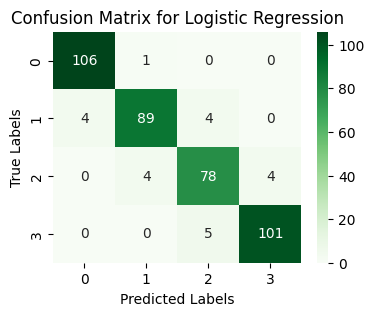
\includegraphics[height=14em]{cmat_LR.png}
        \caption{Confusion Matrix for Logistic Regression}
        \label{cmat_LR}
    \end{minipage}
    \hfill
    \begin{minipage}{0.45\textwidth}
        \centering
        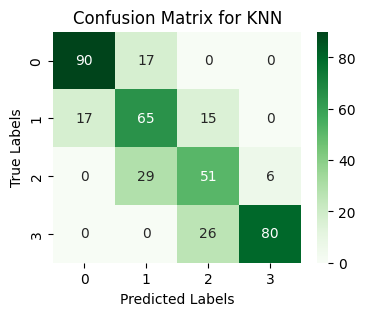
\includegraphics[height=14em]{cmat_KNN.png}
        \caption{Confusion Matrix for K-Nearest Neighbors (KNN)}
        \label{cmat_KNN}
    \end{minipage}
\end{figure}

\begin{figure}[H]
    \centering
		\begin{minipage}{0.45\textwidth}
			\centering
			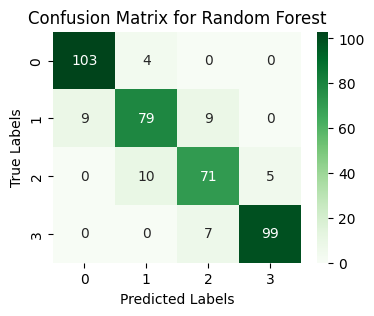
\includegraphics[height=14em]{cmat_RF.png}
			\caption{Confusion Matrix for Random Forest}
			\label{cmat_RF}
		\end{minipage}
    \hfill
    \begin{minipage}{0.45\textwidth}
        \centering
        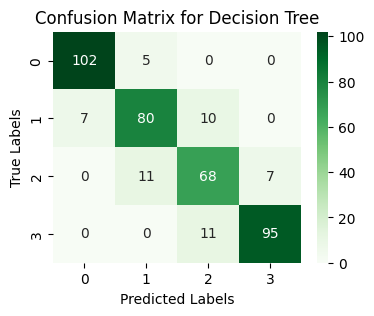
\includegraphics[height=14em]{cmat_DT.png}
        \caption{Confusion Matrix for Decision Tree}
        \label{cmat_DT}
    \end{minipage}
    
\end{figure}

\begin{figure}[H]
    \centering
		\begin{minipage}{0.45\textwidth}
			\centering
			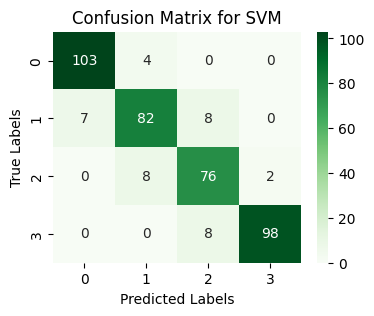
\includegraphics[height=14em]{cmat_SVM.png}
			\caption{Confusion Matrix for Support Vector Machine (SVM)}
			\label{cmat_SVM}
		\end{minipage}
    \hfill
    \begin{minipage}{0.45\textwidth}
        \centering
        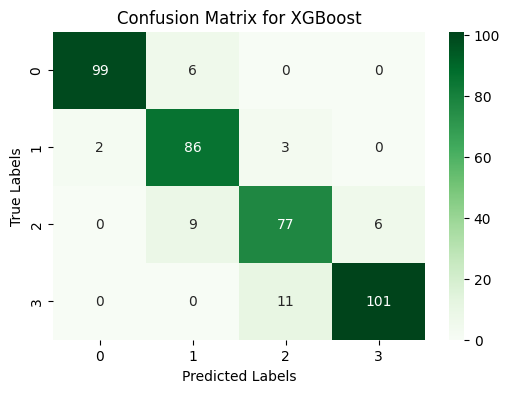
\includegraphics[height=14em]{cmat_XG.png}
        \caption{Confusion Matrix for XGBoost}
        \label{cmat_XG}
    \end{minipage}
\end{figure}
\begin{figure}[H]
    \centering
    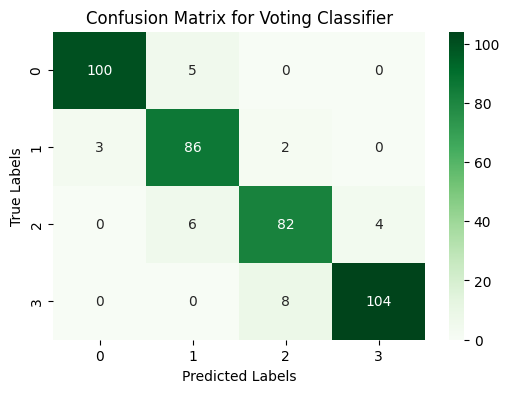
\includegraphics[height=14em]{cmat_VC.png}
    \caption{Confusion Matrix for Voting Classifier}
    \label{cmat_VC}
\end{figure}

\noindent By analyzing these confusion matrices, we observe:
\vspace{-1.25em}
\begin{itemize}
	\setlength\itemsep{-1.05em}
	\item \textbf{Logistic Regression, SVM, and Voting Classifier} should be considered top choices for predicting smartphone prices due to their high accuracy and balanced performance.
	\item \textbf{Random Forest and XGBoost} are also strong contenders and can be used if ensemble methods are preferred.
	\item \textbf{KNN and Decision Tree} may require further tuning or may not be suitable for this specific task due to higher misclassification rates.
\end{itemize}
\section{Evaluation Metrics}
The performance of various machine learning models was evaluated using several metrics are summarized in following Table \ref{table:model_performance}.

\begin{table}[H]
\centering
\begin{tabular}{lccccc}
\toprule
\textbf{Model} & \textbf{Accuracy Train} & \textbf{Accuracy Test} & \textbf{Precision Test} & \textbf{Recall Test} & \textbf{F1-Score Test} \\
\toprule
Logistic Regression & $0.943125$ & $0.9500$ & $0.950751$ & $0.9500$ & $0.950200$ \\
\midrule
KNN & $0.881875$ & $0.7600$ & $0.768319$ & $0.7600$ & $0.762744$ \\
\midrule
Random Forest & $1.000000$ & $0.8950$ & $0.897642$ & $0.8950$ & $0.895610$ \\
\midrule
Decision Tree & $1.000000$ & $0.8425$ & $0.847370$ & $0.8425$ & $0.844235$ \\
\midrule
SVM & $0.951875$ & $0.9175$ & $0.921265$ & $0.9175$ & $0.918080$ \\
\midrule
XGBoost & $1.000000$ & $0.9125$ & $0.913700$ & $0.9125$ & $0.912583$ \\
\midrule
Voting Classifier & $0.970000$ & $0.9150$ & $0.918720$ & $0.9150$ & $0.915258$ \\
\bottomrule
\end{tabular}
\caption{Results for price\_range prediction}
\label{table:model_performance}
\end{table}

\section{Comparison between different Models}
\begin{itemize}
	\setlength\itemsep{-1.05em}
	\item \textbf{Logistic Regression:} Achieved high accuracy on both training ($0.943125$) and test ($0.9500$) sets, indicating good generalization. Precision, recall, and F1-score are also high, making it a reliable model for this task.
	\item \textbf{KNN:} Showed moderate performance with a test accuracy of $0.7600$. The lower precision, recall, and F1-score suggest that KNN may not be the best choice for this dataset.
	\item \textbf{Random Forest:} Exhibited perfect training accuracy ($1.000000$) but lower test accuracy ($0.8950$), indicating potential overfitting. However, it still performed well on the test set with good precision, recall, and F1-score.
	\item \textbf{Decision Tree:} Similar to Random Forest, it showed perfect training accuracy ($1.000000$) but lower test accuracy ($0.8425$), suggesting overfitting. The precision, recall, and F1-score are also lower compared to Random Forest.
	\item \textbf{SVM:} Demonstrated strong performance with high accuracy on both training ($0.951875$) and test ($0.9175$) sets. The high precision, recall, and F1-score indicate that SVM is a robust model for this task.
	\item \textbf{XGBoost:} Achieved perfect training accuracy ($1.000000$) and high test accuracy ($0.9125$). The precision, recall, and F1-score are also high, making it a strong contender for this task.
	\item \textbf{Voting Classifier:} Combined the strengths of multiple models, resulting in high test accuracy ($0.9150$) and strong precision, recall, and F1-score. This ensemble method provides a balanced and accurate prediction system.
\end{itemize}

\chapter{Discussion}
\section{Analysis of Results}
\section{Anomalies and Unexpected Findings}
The dataset we chose did not have any class imbalances but there may have been challenges related to it, which can affect model predictions, particularly in underrepresented categories. \\
Also we found that among the 19 features, 13 were not much important such as 3G, 4G, front and primary camera quality, and screen resolution components. Removing redundant features improved model performance and reduced complexity. \\	
\section{Limitations}
\vspace{-0.5em}
\begin{itemize}
	\setlength\itemsep{-1.25em}
	\item  If certain price categories were underrepresented, the model might not perform equally well across all classes, potentially favoring more common categories.
	\item The impact of feature selection and engineering steps could vary, and further refinement might be needed to capture more complex relationships in the data.
	\item The results might not generalize well to unseen data if there were biases in the dataset or if the training set wasn't diverse enough.
\end{itemize}

\chapter{Conclusion}
\section{Key Takeaways}
The key takeaways from this project are:
\vspace{-1.25em}
\begin{itemize}
	\setlength\itemsep{-1.05em}
	\item The project successfully developed a classification model capable of categorizing smartphones into distinct price segments (Low, Medium, High, Very High) using a variety of machine learning algorithms.
	\item A thorough feature analysis revealed the most influential factors for predicting smartphone prices, such as RAM, battery power, and camera quality.
	\item The systematic feature selection process, including normalization and encoding, highlighted critical features that contributed significantly to model accuracy.
	\item Effective feature engineering, including normalization of screen and pixel areas, ensured a refined and optimized dataset for training.
	\item Various machine learning models were implemented, tuned, and evaluated. Metrics such as accuracy, precision, and recall were used to compare the models.
	\item The project provided clear insights into which algorithms were more effective for this classification task. For example, ensemble methods like the Voting Classifier generally outperformed individual classifiers.
	\item The utilization of metrics like confusion matrices, ROC curves, and AUC scores provided a comprehensive understanding of the model’s accuracy and reliability.
	\item The project made methodological contributions by developing a replicable framework for smartphone price categorization, emphasizing feature analysis and multi-algorithm comparison.
	\item The workflow established in this project serves as a template for future predictive modeling challenges, particularly in consumer market analysis using machine learning techniques.
\end{itemize}
\section{Reflection on Objectives}
\vspace{-0.5em}
\begin{enumerate}
	\setlength\itemsep{-1.05em}
	\item{\textbf{Robust Classification Model :}}
	      \vspace{-1.65em}
	      \begin{itemize}
		      \setlength\itemsep{-1.5em}
		      \item The project met its objective of building an accurate classification model, using multiple algorithms and optimizing them for high predictive accuracy.
		      \item The most significant features influencing smartphone pricing were identified, meeting the goal of leveraging key variables for prediction.
	      \end{itemize}
	\item{\textbf{Feature Analysis and Selection :}}
	      \vspace{-1.65em}
	      \begin{itemize}
		      \setlength\itemsep{-1.5em}
		      \item A comprehensive feature analysis was performed, and a systematic approach to feature selection was developed, successfully identifying the most influential smartphone attributes.
		      \item The selection of relevant features directly impacted the model’s performance, aligning with the project’s goals.
	      \end{itemize}
	\item{\textbf{Comparative Algorithm Performance :}}
	      \vspace{-1.65em}
	      \begin{itemize}
		      \setlength\itemsep{-1.5em}
		      \item Multiple machine learning algorithms were tested, and their performances were compared, allowing for the selection of the most effective model for smartphone categorization.
		      \item The comparison revealed insights into which algorithms handled the dataset’s characteristics best, achieving the project’s objective of comparative analysis.
	      \end{itemize}
	\item{\textbf{Practical Applicability :}}
	      \vspace{-1.65em}
	      \begin{itemize}
		      \setlength\itemsep{-1.5em}
		      \item The practical utility of the model was demonstrated, showcasing how it could assist both manufacturers and consumers in making data-driven decisions, achieving this core objective.
	      \end{itemize}
	\item{\textbf{Methodological Contribution :}}
	      \vspace{-1.65em}
	      \begin{itemize}
		      \setlength\itemsep{-1.5em}
		      \item A replicable methodology was established, contributing to market analysis using machine learning. The project’s systematic approach, from feature analysis to model comparison, stands as a reference for similar challenges.
	      \end{itemize}
\end{enumerate}
\section{Future Work}
\vspace{-0.5em}
\begin{enumerate}
	\setlength\itemsep{-1.05em}
	\item{\textbf{Addressing Class Imbalances: }}
	      \vspace{-1.65em}
	      \begin{itemize}
		      \setlength\itemsep{-1.5em}
		      \item Future research could focus on balancing the dataset more effectively, employing techniques like SMOTE (Synthetic Minority Over-sampling Technique) to handle underrepresented categories.
		      \item Experimenting with different sampling strategies or cost-sensitive algorithms might yield better performance across all price segments.
	      \end{itemize}
	\item{\textbf{Advanced Feature Engineering: }}
	      \vspace{-1.65em}
	      \begin{itemize}
		      \setlength\itemsep{-1.5em}
		      \item Introducing more sophisticated feature engineering methods, such as polynomial features or interaction terms, might capture deeper relationships between variables.
		      \item Incorporating external data sources like user reviews or brand reputation could provide additional features for enhanced model predictions.
	      \end{itemize}
	\item{\textbf{Deep Learning Approaches:	}}
	      \vspace{-1.65em}
	      \begin{itemize}
		      \setlength\itemsep{-1.5em}
		      \item Exploring deep learning models, such as neural networks, could help capture complex patterns in the data that traditional machine learning models might miss.
		      \item Fine-tuning deep learning algorithms might lead to better generalization and improved accuracy for smartphone price prediction.
	      \end{itemize}
	\item{\textbf{Model Interpretability:	:}}
	      \vspace{-1.65em}
	      \begin{itemize}
		      \setlength\itemsep{-1.5em}
		      \item Enhancing model interpretability by using techniques like SHAP (Shapley Additive Explanations) or LIME (Local Interpretable Model-agnostic Explanations) can provide more insights into how predictions are made, especially for complex models.
	      \end{itemize}
	\item{\textbf{Expanding Practical Use Cases:	}}
	      \vspace{-1.65em}
	      \begin{itemize}
		      \setlength\itemsep{-1.5em}
		      \item Future work could extend beyond categorization, such as predicting the price value itself or identifying which features drive consumer satisfaction.
		      \item The developed model can be adapted to other product categories, providing a broader application in market analysis and consumer research.
	      \end{itemize}
\end{enumerate}

\renewcommand{\bibname}{References}
\begin{thebibliography}{9}
	\bibitem{hadsonml}
	Géron, Aurélien. \textit{Hands-On Machine Learning with Scikit-Learn, Keras, and TensorFlow}. 3rd ed., O'Reilly Media, 2023.

	\bibitem{asim2018}
	Asim, Muhammad, and Zafar Khan. "Mobile Price Class Prediction Using Machine Learning Techniques." \textit{International Journal of Computer Applications}, March 2018. DOI: \texttt{10.5120/ijca2018916555}.

	\bibitem{chandrashekhara2019}
	Chandrashekhara, K. T., and M. Thungamani. "Smartphone Price Prediction in Retail Industry Using Machine Learning Techniques." In \textit{Emerging Research in Electronics, Computer Science and Technology, Lecture Notes in Electrical Engineering 545}, edited by V. Sridhar et al., Springer Nature Singapore Pte Ltd., 2019. DOI: \texttt{10.1007/978-981-13-5802-9\_34}.

	\bibitem{ercan2023}
	Ercan \&  Şimşek, "Mobile Phone Price Classification Using Machine Learning." \textit{International Journal of Advanced Natural Sciences and Engineering Researches}, vol. 7, no. 4, 2023, pp. 458-462. DOI: \texttt{10.59287/ijanser.791}.

	\bibitem{abbasi2024}
	Abbasi, Muhammad Hasnain, Abdul Sajid, Muhammad Arshad Awan, and Ayeb Amani. "Predicting The Price Of Used Electronic Devices Using Machine Learning Techniques." \textit{International Journal of Computing and Related Technologies}, vol. 4, no. 1, 2024. Available at: \texttt{https://www.researchgate.net/publication/377526585}.

	\bibitem{gupta2020}
	Gupta, Akash, and Suhasini Kottur. "Mobile Price Prediction by Its Features Using Predictive Model of Machine Learning." \textit{UGC Care Journal}, August 2020. DOI: \texttt{10.13140/RG.2.2.20054.52800}.

	\bibitem{kumuda2021}
	Kumuda S, Vishal Karur, and Karthick Balaje S. E. "Prediction of Mobile Model Price Using Machine Learning Techniques." \textit{International Journal of Engineering and Advanced Technology (IJEAT)}, vol. 11, no. 1, October 2021. DOI: \texttt{10.35940/ijeat.A3219.1011121}.

\end{thebibliography}
\addcontentsline{toc}{chapter}{References}

\end{document}